% Latex template: mahmoud.s.fahmy@students.kasralainy.edu.eg
% For more details: https://www.sharelatex.com/learn/Beamer

\documentclass{beamer}					% Document class
\geometry{papersize={15cm,10cm}}

\setbeamertemplate{footline}[text line]{%
  \parbox{\linewidth}{\vspace*{-8pt}\hfill\hfill\insertpagenumber}}
\setbeamertemplate{navigation symbols}{}

\usepackage[english]{babel}				% Set language
\usepackage[utf8x]{inputenc}			% Set encoding

\mode<presentation>						% Set options
{
  \usetheme{default}					% Set theme
  \usecolortheme{default} 				% Set colors
  \usefonttheme{default}  				% Set font theme
  \setbeamertemplate{caption}[numbered]	% Set caption to be numbered
}

% Uncomment this to have the outline at the beginning of each section highlighted.
%\AtBeginSection[]
%{
%  \begin{frame}{Outline}
%    \tableofcontents[currentsection]
%  \end{frame}
\usepackage{graphicx}					% For including figures
\usepackage{booktabs}					% For table rules
\usepackage{hyperref}	
\usepackage{tikz-network}				% For cross-referencing
\usepackage[absolute,overlay]{textpos}
\usepackage{bm}
\usepackage[font=small,labelfont=bf]{caption}				% For cross-referencing

\title{Visualizing nucleosome cluster dynamics with dense single molecule localization microscopy}	% Presentation title
\author{Clayton W. Seitz}								% Presentation author
\date{\today}									% Today's date	

\begin{document}

% Title page
% This page includes the informations defined earlier including title, author/s, affiliation/s and the date
\begin{frame}
  \titlepage
\end{frame}


% The following is the most frequently used slide types in beamer
% The slide structure is as follows:
%
%\begin{frame}{<slide-title>}
%	<content>
%\end{frame}


\begin{frame}
\frametitle{}
\centering
\Large \textcolor{black}{Introduction}
\end{frame}

\begin{frame}{Summary}
\begin{itemize}
\item We study the organization of nucleosomes in living cells, and I am interested in the impact of BRD4 phase separation (fusion/fission) on chromatin packing, as previous work has shown chromatin nanodomains are highly dynamic structures (Barth 2020)
\item We study chromatin structure using SMLM, which can increase lateral resolution by one order of magnitude in living cells compared to standard widefield microscpy
\item  SMLM enables simultaneous super-resolution of chromatin structure and single molecule tracking to probe the physical properties of chromatin nanodomins

\item In general, the uncertainty of a statistical estimator in SMLM determines the resolution limit (Cramer-Rao lower bound). \item Deep learning can generalize SMLM to three dimensions, particularly in sparsely labeled regimes

\item SMLM achieves the highest resolution of SR methods; however, there is a fundamental tradeoff between spatial and temporal resolution (Shroff et al)

\item Therefore, we look to other alternatives for resolution enhancement which combine the power of deep image translation methods e.g., ANNA-PALM
\end{itemize}
\end{frame}


\begin{frame}
\frametitle{Instrumentation for super-resolution and high throughput microscopy}

\begin{figure}
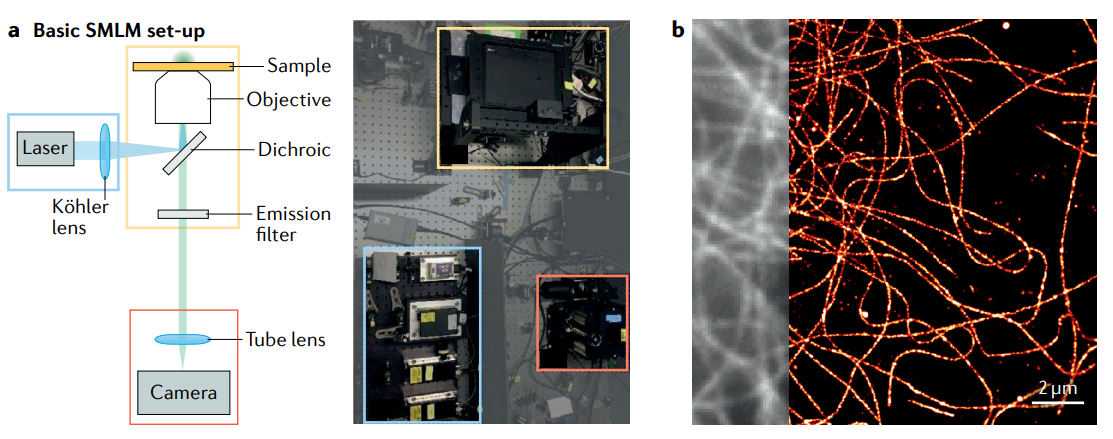
\includegraphics[width=12cm]{Setup.png}
\end{figure}
  
\end{frame}

\begin{frame}
\frametitle{The photophysics of rhodamines}

\begin{figure}
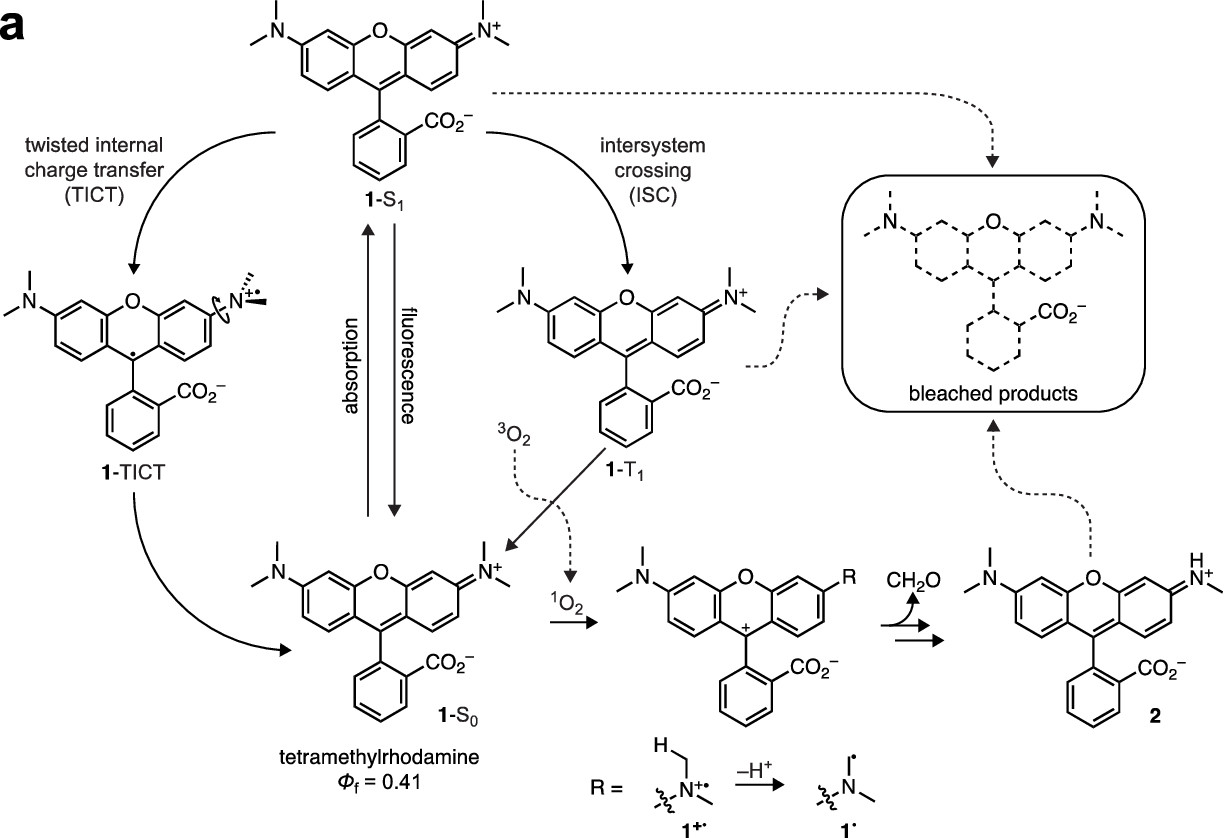
\includegraphics[width=10cm]{Rhodamines.png}
\end{figure}
\begin{itemize}
\item  Reduction of the T1 state yields a dark, long-lived, and stable radical state
\item The reducing agent is usually a primary thiol like cysteamine (MEA)
\end{itemize}
\end{frame}

\begin{frame}{The OFF state of JF646 can be maintained with high laser power}
\begin{textblock*}{11cm}(1.5cm,1.3cm)
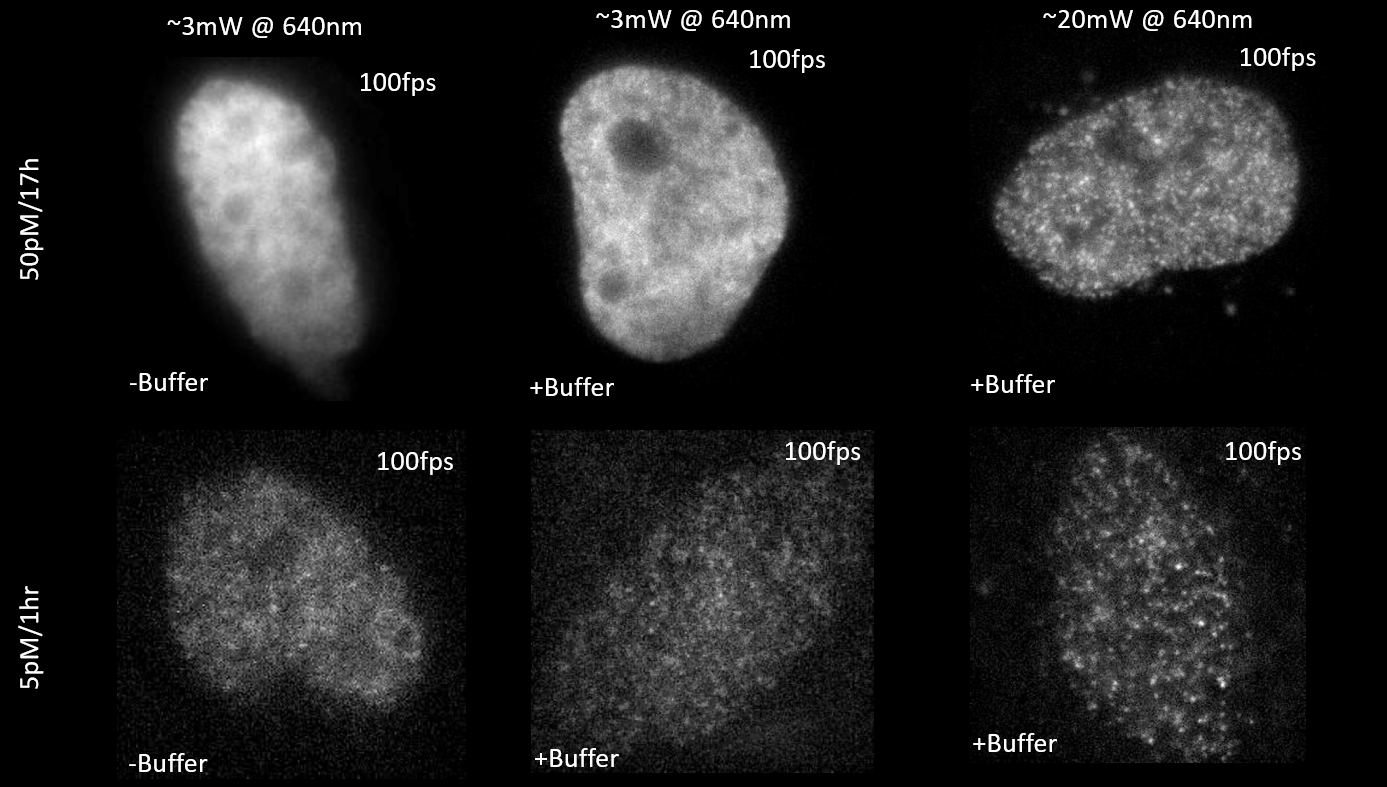
\includegraphics[width=11cm]{Laser.png}
\end{textblock*}
\begin{textblock*}{\textwidth}(0.5cm,8.0cm)
\begin{itemize}
\item SMLM is desirable for SR due to very high res and no scanning (STED)
\item Less control over photophysical state, but high throughput
\item High power compensates for dense labeling
\end{itemize}
\end{textblock*}
\end{frame}


\begin{frame}{Maximum likelihood localization of an isolated fluorescent emitter}
Localization: $\theta^{*} = \underset{\theta}{\mathrm{argmax}}\prod_{k}P(H_{k}|\theta)= \underset{\theta}{\mathrm{argmin}}-\sum_{k}\log P(H_{k}|\theta)$

\begin{textblock*}{8cm}(6.5cm,2.5cm)
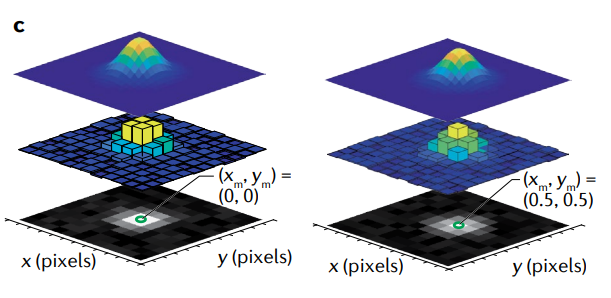
\includegraphics[width=\textwidth]{Model.png}
\end{textblock*}

\begin{textblock*}{2cm}(1cm,2.5cm)
\begin{align*}
\mu_{k} &= g_{k}\textcolor{red}{\eta} \textcolor{cyan}{N_{0}}\textcolor{blue}{\Delta}\int_{\mathrm{pixel}} G(x,y)dA\\
\\
\textcolor{red}{\eta} &- \mathrm{quantum\; efficiency}\\
\textcolor{cyan}{N_{0}} &- \mathrm{emission\; rate}\\
\textcolor{blue}{\Delta} &- \mathrm{exposure\; time}
\end{align*}
\end{textblock*}


\vspace{2in}

\begin{equation*}
P(H_{k}|\theta) = A\sum_{q=0}^{\infty} \frac{1}{q!}e^{-\mu_{k}}\mu_{k}^{q}\frac{1}{\sqrt{2\pi}\sigma_{k}}e^{-\frac{(H_{k}-g_{k}q-o_{k})}{2\sigma_{k}^{2}}}
\end{equation*}
\\
$P(H_{k}|\theta)$ can be approximated as Poisson at high signal-to-noise ($\mathrm{SNR}$)

\end{frame}

\begin{frame}{A Poisson approximation at moderate SNR simplifies SMLM}

\begin{figure}
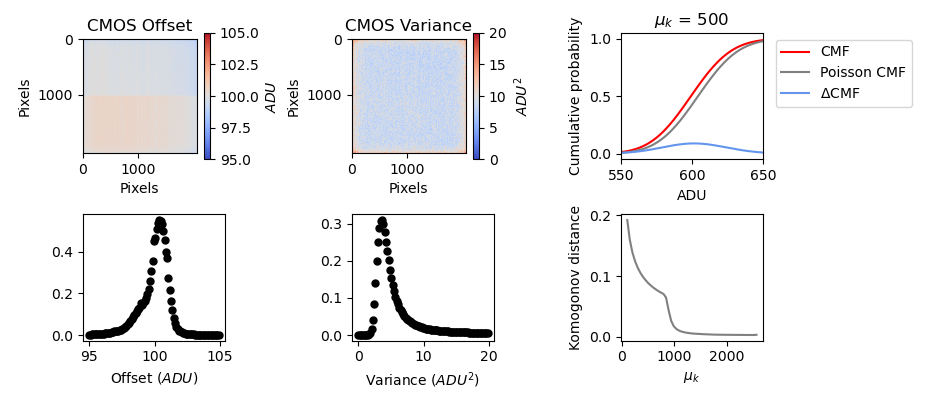
\includegraphics[width=13cm]{Noise.png}
\end{figure}

\begin{itemize}
\item $P(H_{k}-o_{k}|\theta) = \mathrm{Poisson}(\mu_{k}+\sigma_{k}^{2}|\theta)$ for pixel offset $o_{k}$ noise variance $\sigma_{k}^{2}$
\item Fisher information and Cramer-Rao lower bound (CRLB) can be computed analytically for Poisson log-likelihood $\ell$ (Smith 2010, Huang 2013)
\end{itemize} 
 
\end{frame}

\begin{frame}{Estimator precision sets the resolution limit in localization microscopy}
\begin{textblock*}{4cm}(1.0cm,1.0cm)
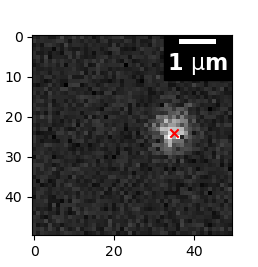
\includegraphics[width=4cm]{MCMC/Figure_1.png}
\end{textblock*}
\begin{textblock*}{4cm}(1.0cm,5cm)
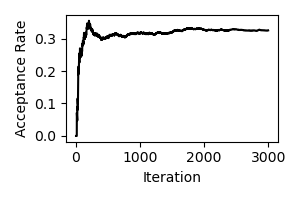
\includegraphics[width=4cm]{MCMC/Figure_2.png}
\end{textblock*}
\begin{textblock*}{9cm}(5cm,1.0cm)
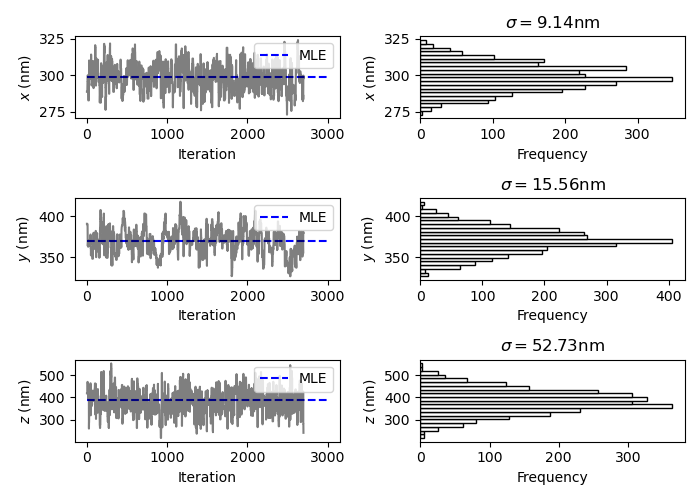
\includegraphics[width=9cm]{MCMC/Figure_3.png}
\end{textblock*}
\begin{textblock*}{13cm}(0.5cm,8cm)
\begin{itemize}
\item Variance of the posterior $P(\theta|\vec{H})$ is a suitable particle filter
\item We assume uniform priors on coordinates
\end{itemize}
\end{textblock*}
\end{frame}

\begin{frame}{Estimator precision sets the resolution limit in 2D}
\begin{figure}
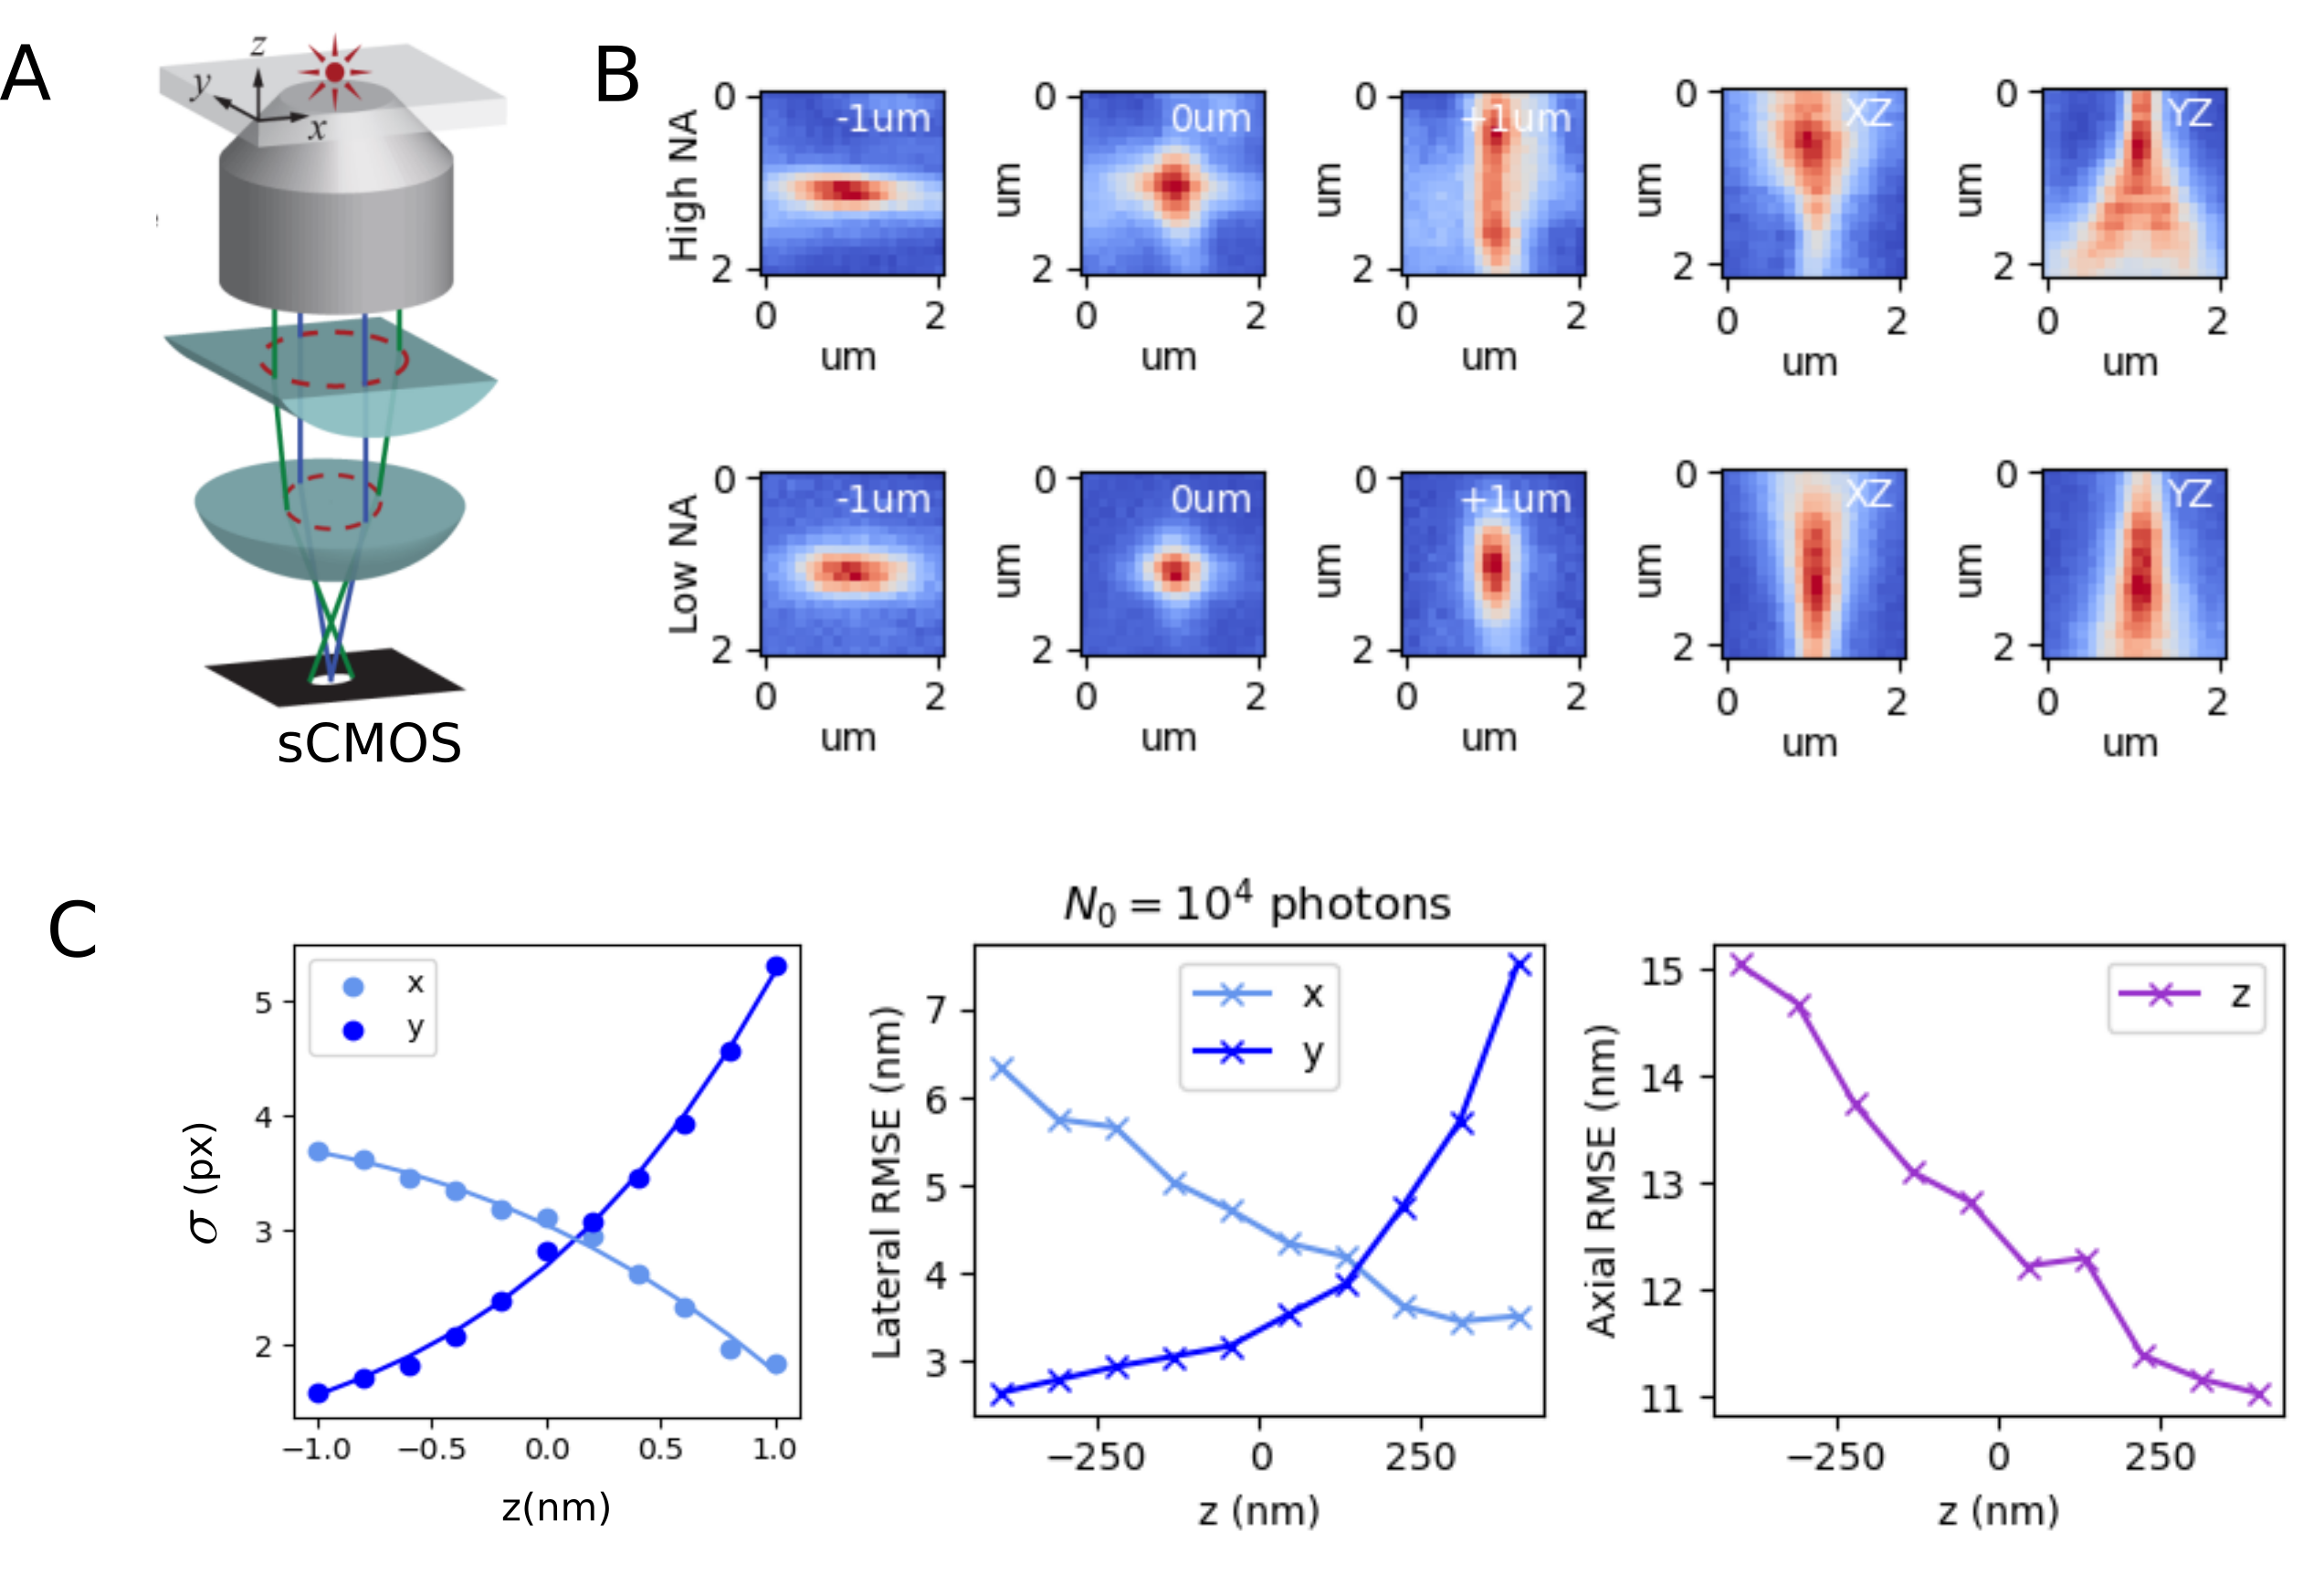
\includegraphics[width=11cm]{Astigmatism.png}
\end{figure}
\begin{itemize}
\item RMSE of is a quality metric of a localization estimator
\item The RMSE is bounded from below by the CRLB
\end{itemize}
\end{frame}


\begin{frame}{Estimator precision sets the resolution limit in 3D}
\begin{figure}
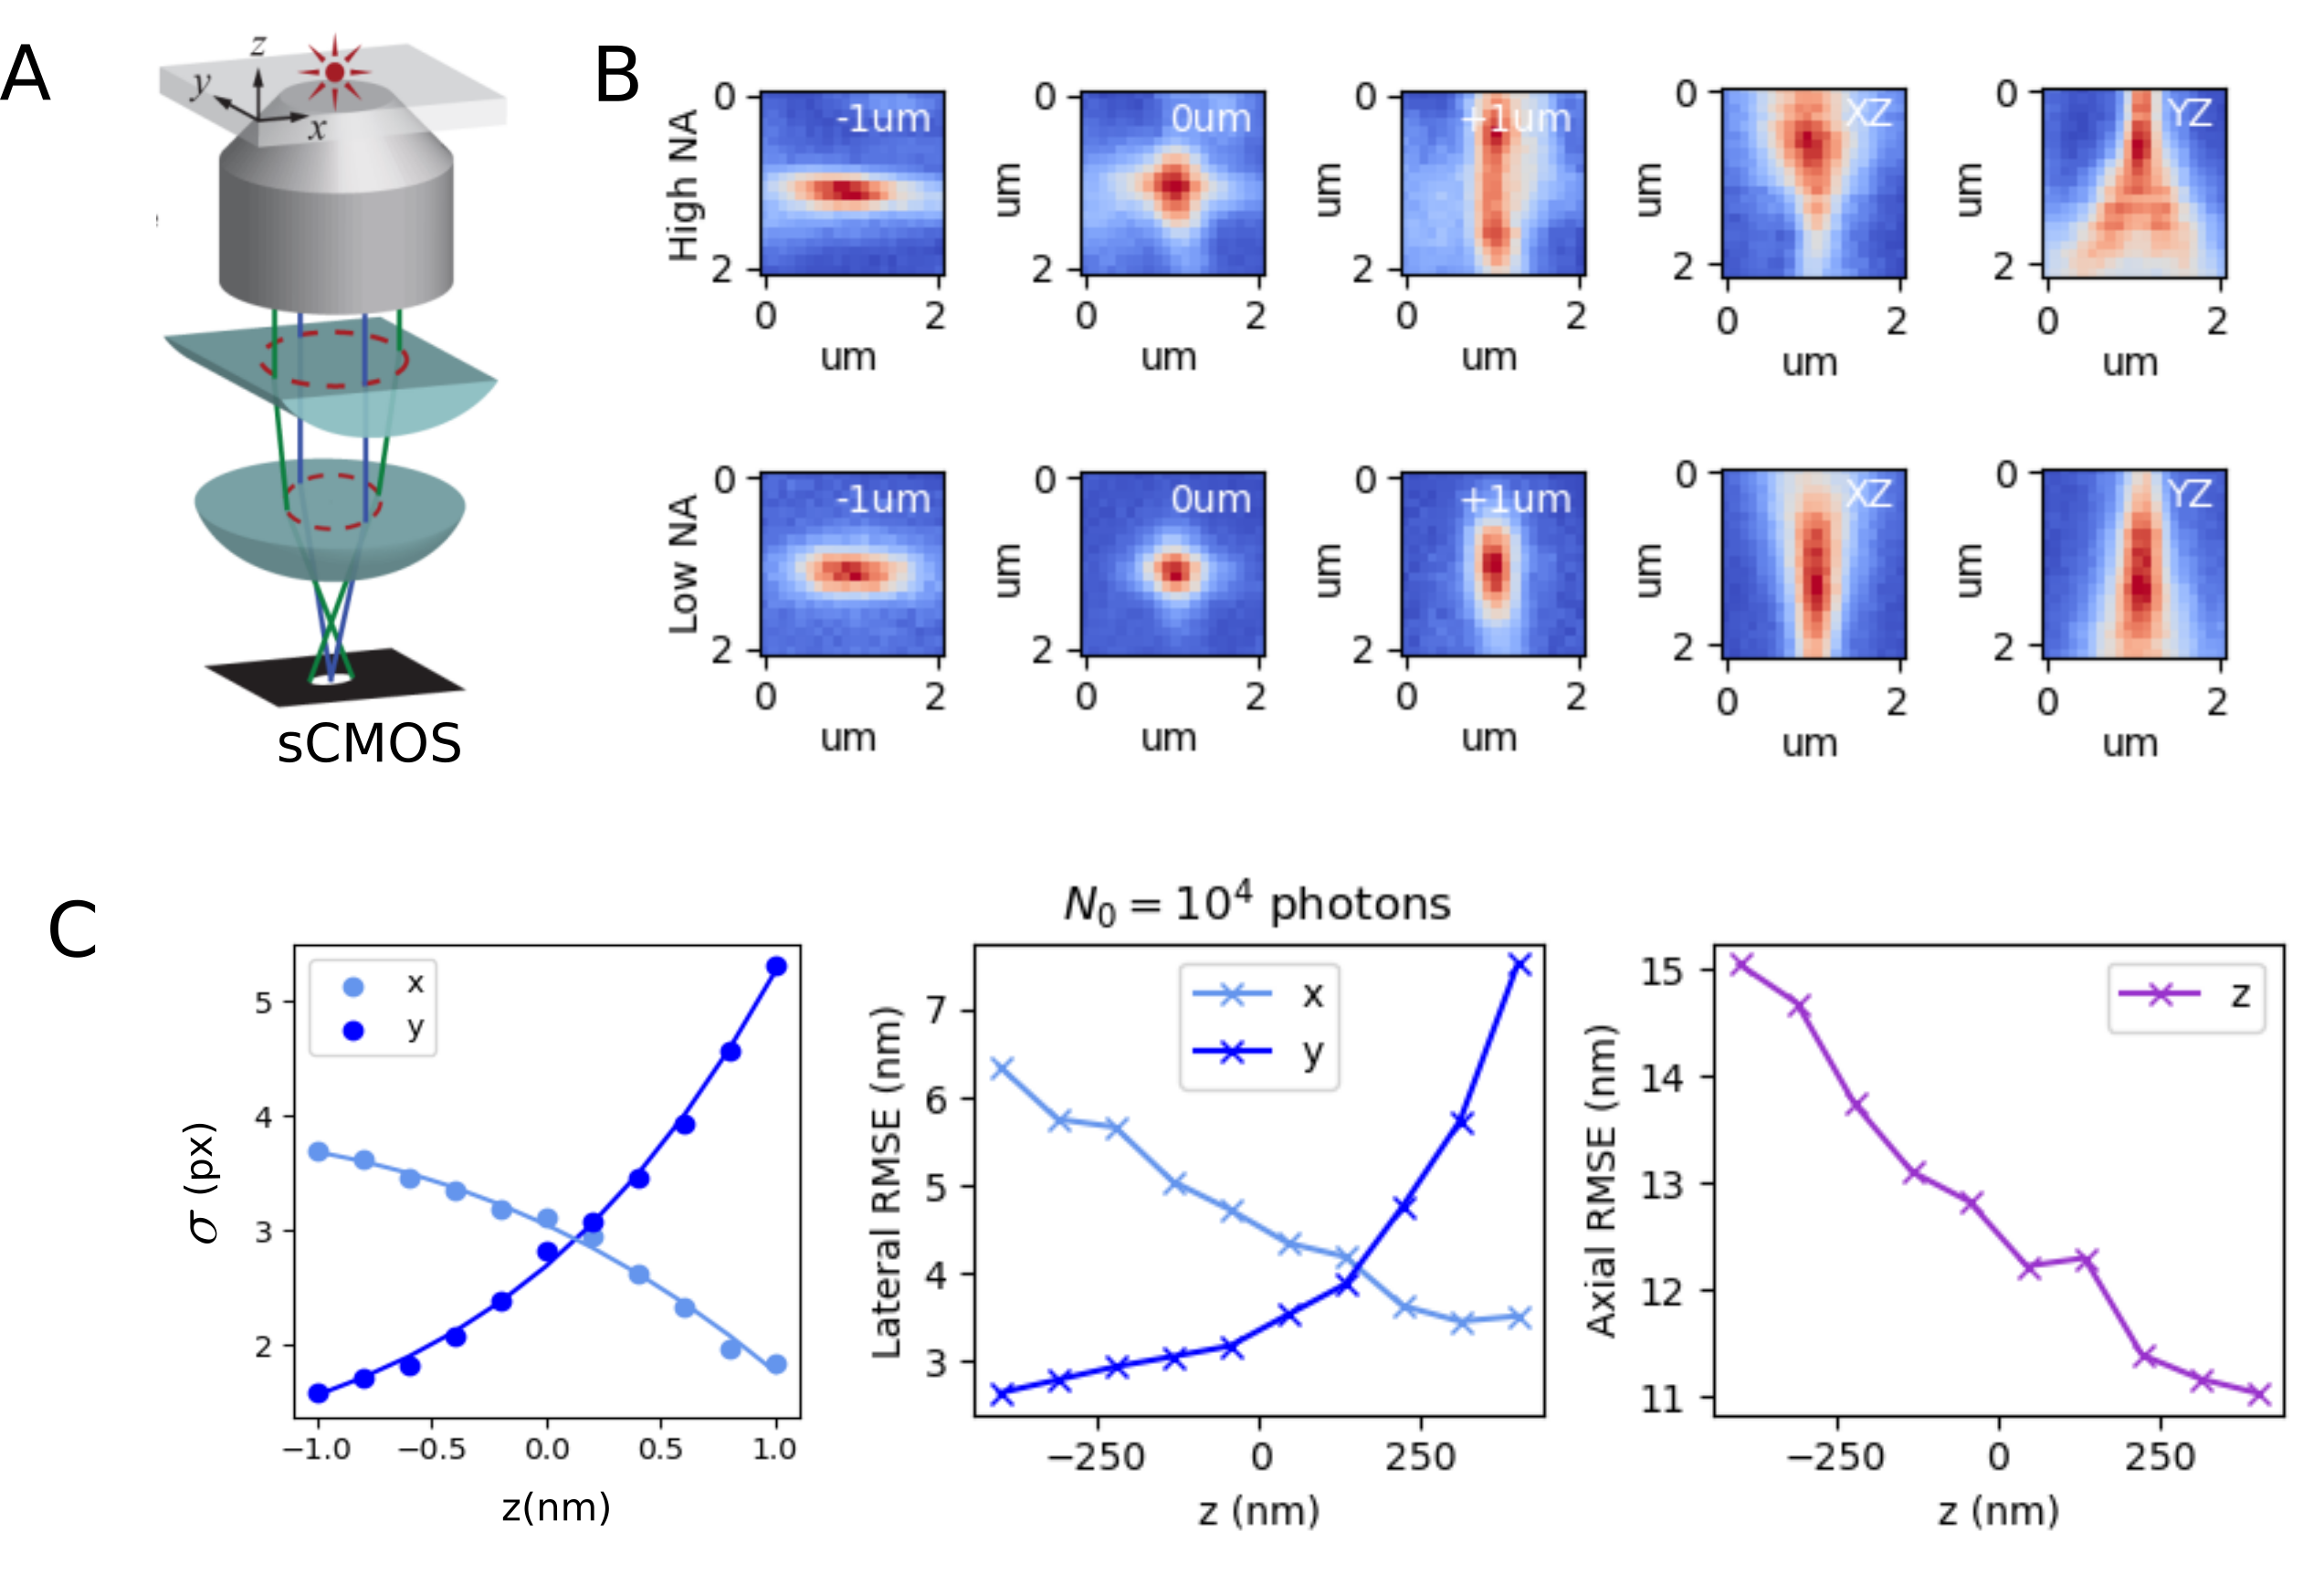
\includegraphics[width=11cm]{Astigmatism.png}
\end{figure}
\begin{itemize}
\item A weak ($f=10$m) cylindrical lens breaks the axial symmetry of the PSF
\end{itemize}
\end{frame}


\begin{frame}{The tradeoff between spatial and temporal resolution in SMLM}
\begin{figure}
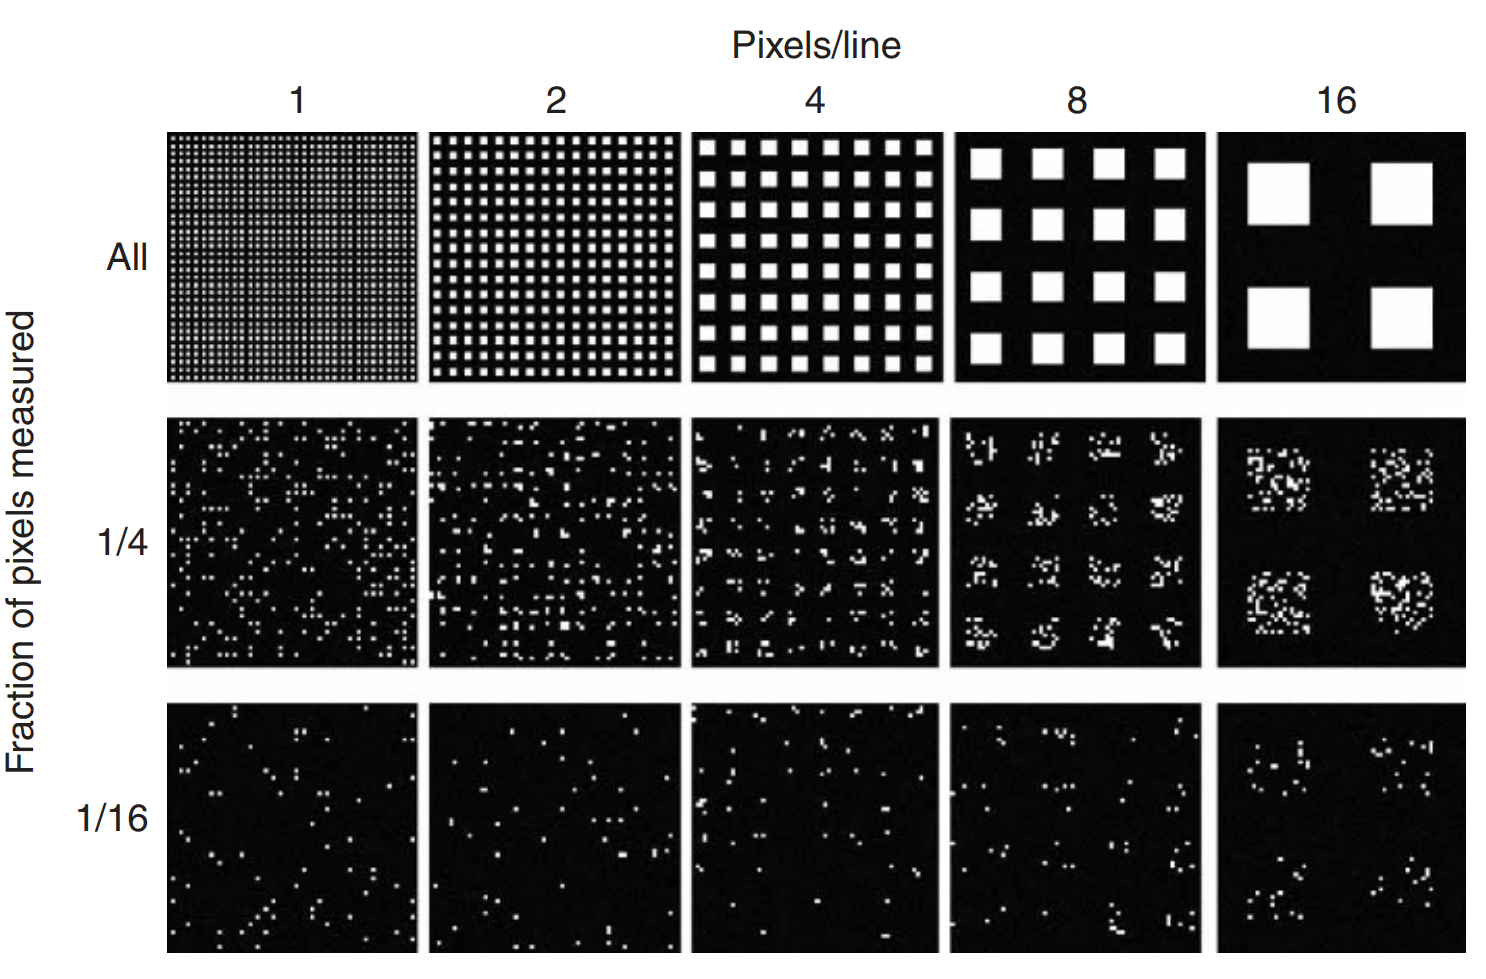
\includegraphics[width=10cm]{Shroff.png}
\end{figure}
\textit{Shroff et al. Live-cell photoactivated localization microscopy of
nanoscale adhesion dynamics. Nature Methods.}
\end{frame}


\begin{frame}{The tradeoff between spatial and temporal resolution in SMLM}
\begin{figure}
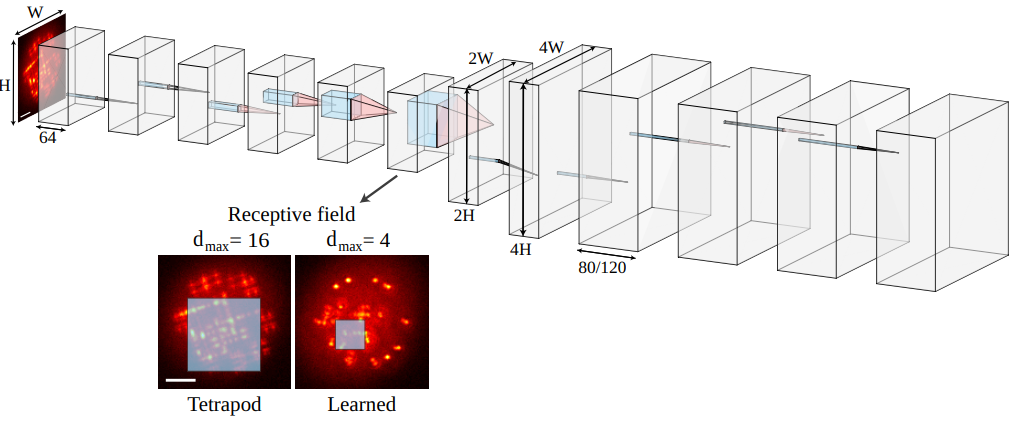
\includegraphics[width=13cm]{Architecture.png}
\end{figure}
\begin{itemize}
\item ANNA-PALM (Ouyang 2018) use prior information to generate SR images from fewer localizations
\item DECODE (Speiser 2021) and DeepSTORM3D (Nehme 2020) instead process dense images to increase localizations per unit time
\end{itemize}
\end{frame}

\begin{frame}{Deep learning can generalize precise SMLM to three dimensions}
\begin{figure}
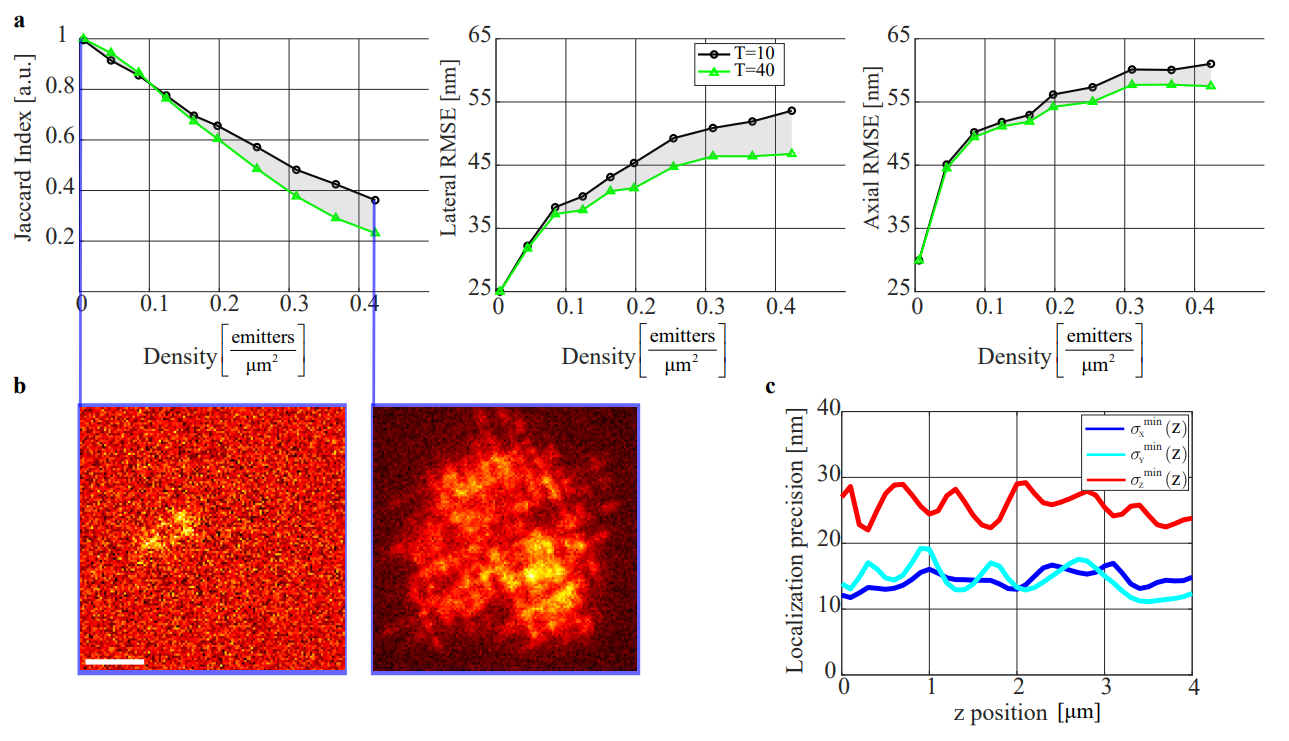
\includegraphics[width=12cm]{Jaccard.png}
\end{figure}
Several methods have been designed to break the time-resolution barrier
\begin{itemize}
\item Density estimation using 30x30nm bins
\item Bayesian information criterion (BIC) used to reduce the effect of multiple blinking, assuming 10nm lateral uncertainty
\end{itemize}
\end{frame}


\begin{frame}{Chromatin nanodomains in a living Hela cell nucleus at 37C}

\begin{textblock*}{13cm}(0.5cm,1.5cm)
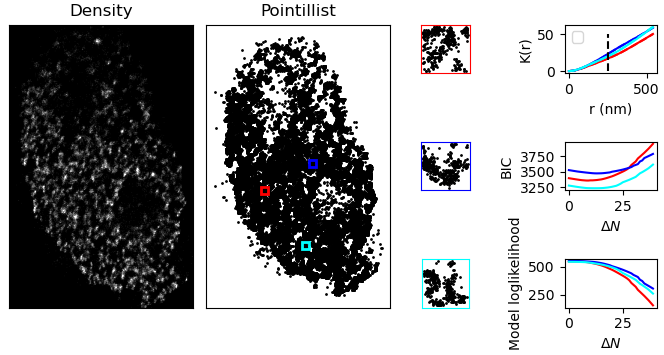
\includegraphics[width=\textwidth]{Cluster.png}
\end{textblock*}

\begin{textblock*}{13cm}(0.5cm,8.25cm)
\begin{itemize}
\item Density estimation using 30x30nm bins
\item Bayesian information criterion (BIC) used to reduce the effect of multiple blinking, assuming 10nm lateral uncertainty
\end{itemize}
\end{textblock*}

\end{frame}

\begin{frame}{Diffusion increases localization uncertainty in live-cell SMLM}

Nucleosome diffusion has been modeled in various potentials:
\vspace{0.1in}
\begin{itemize}
\item Bead model: $V(r_{ij}) = \epsilon_{0}(r_{0}/r_{ij})^{12}-\epsilon_{ij}(r_{0}/r_{ij})^{6}$ (Ashwin 2019)
\item Harmonic: $V(\vec{\Delta r}) = \frac{1}{2}k|\vec{\Delta r}|^{2}$ (XXX)
\end{itemize}
\vspace{0.1in}
The latter is attractive because the stationary distribution of Brownian motion in a Harmonic potential is known:


\begin{equation*}
\partial_{t}P(r) = \hat{\mathcal{L}}_{FP}P(r); \hat{\mathcal{L}}_{FP} = \hat{\mathcal{L}}_{FP} = \left(-\frac{\partial}{\partial x}M^{(1)}(t) + \frac{1}{2}\frac{\partial^{2}}{\partial x^{2}}M^{(2)}(t)\right)
\end{equation*}


\begin{equation*}
x',t'|x,t = \mathcal{N}(\mu,\Sigma)
\end{equation*}

\end{frame}

\begin{frame}{Resolution is dependent on photoswitching kinetics}

A molecule is considered "detected" in principle if the measured ADU signal satisfies $\tilde{s} =\mu\tau \geq \delta$ where $\delta$ is a number of photons which satisfy a criterion on localization accuracy.

\begin{equation*}
\alpha = \int_{\delta}^{\Delta}\left(\sum_{n=0}^{\infty}Q(N=n)\psi(\tau|n;\vec{k})\right)d\tau \approx \underset{\tau\sim P(\tau)}{\mathbb{E}}\left(\mathbb{I}[\tau > \delta]\right)
\end{equation*}

$P(\tau)$ is usually obtained by Monte Carlo simulation. This is useful for computing density measures and the total acqusition time:

\begin{equation*}
D = \alpha K\left(\frac{\lambda}{2\mathrm{NA}}\right)\;\; T = \left(\Delta_{SR}+\frac{2N}{\log(1-\alpha)}\right)^{2}
\end{equation*}

For actually inferring $k_{1},k_{2}$, we need a measure of distance between $P(\tilde{s})$ and $P(s|k_{1},k_{2})$ for many $k_{1},k_{2}$ pairs. Luckily we only need to compute $P(s|k_{1},k_{2})$ once, and we can then perform a grid search

\end{frame}

\begin{frame}{Validaton of JQ1 efficacy for BRD4 inhibition in Hela cells}
\begin{figure}
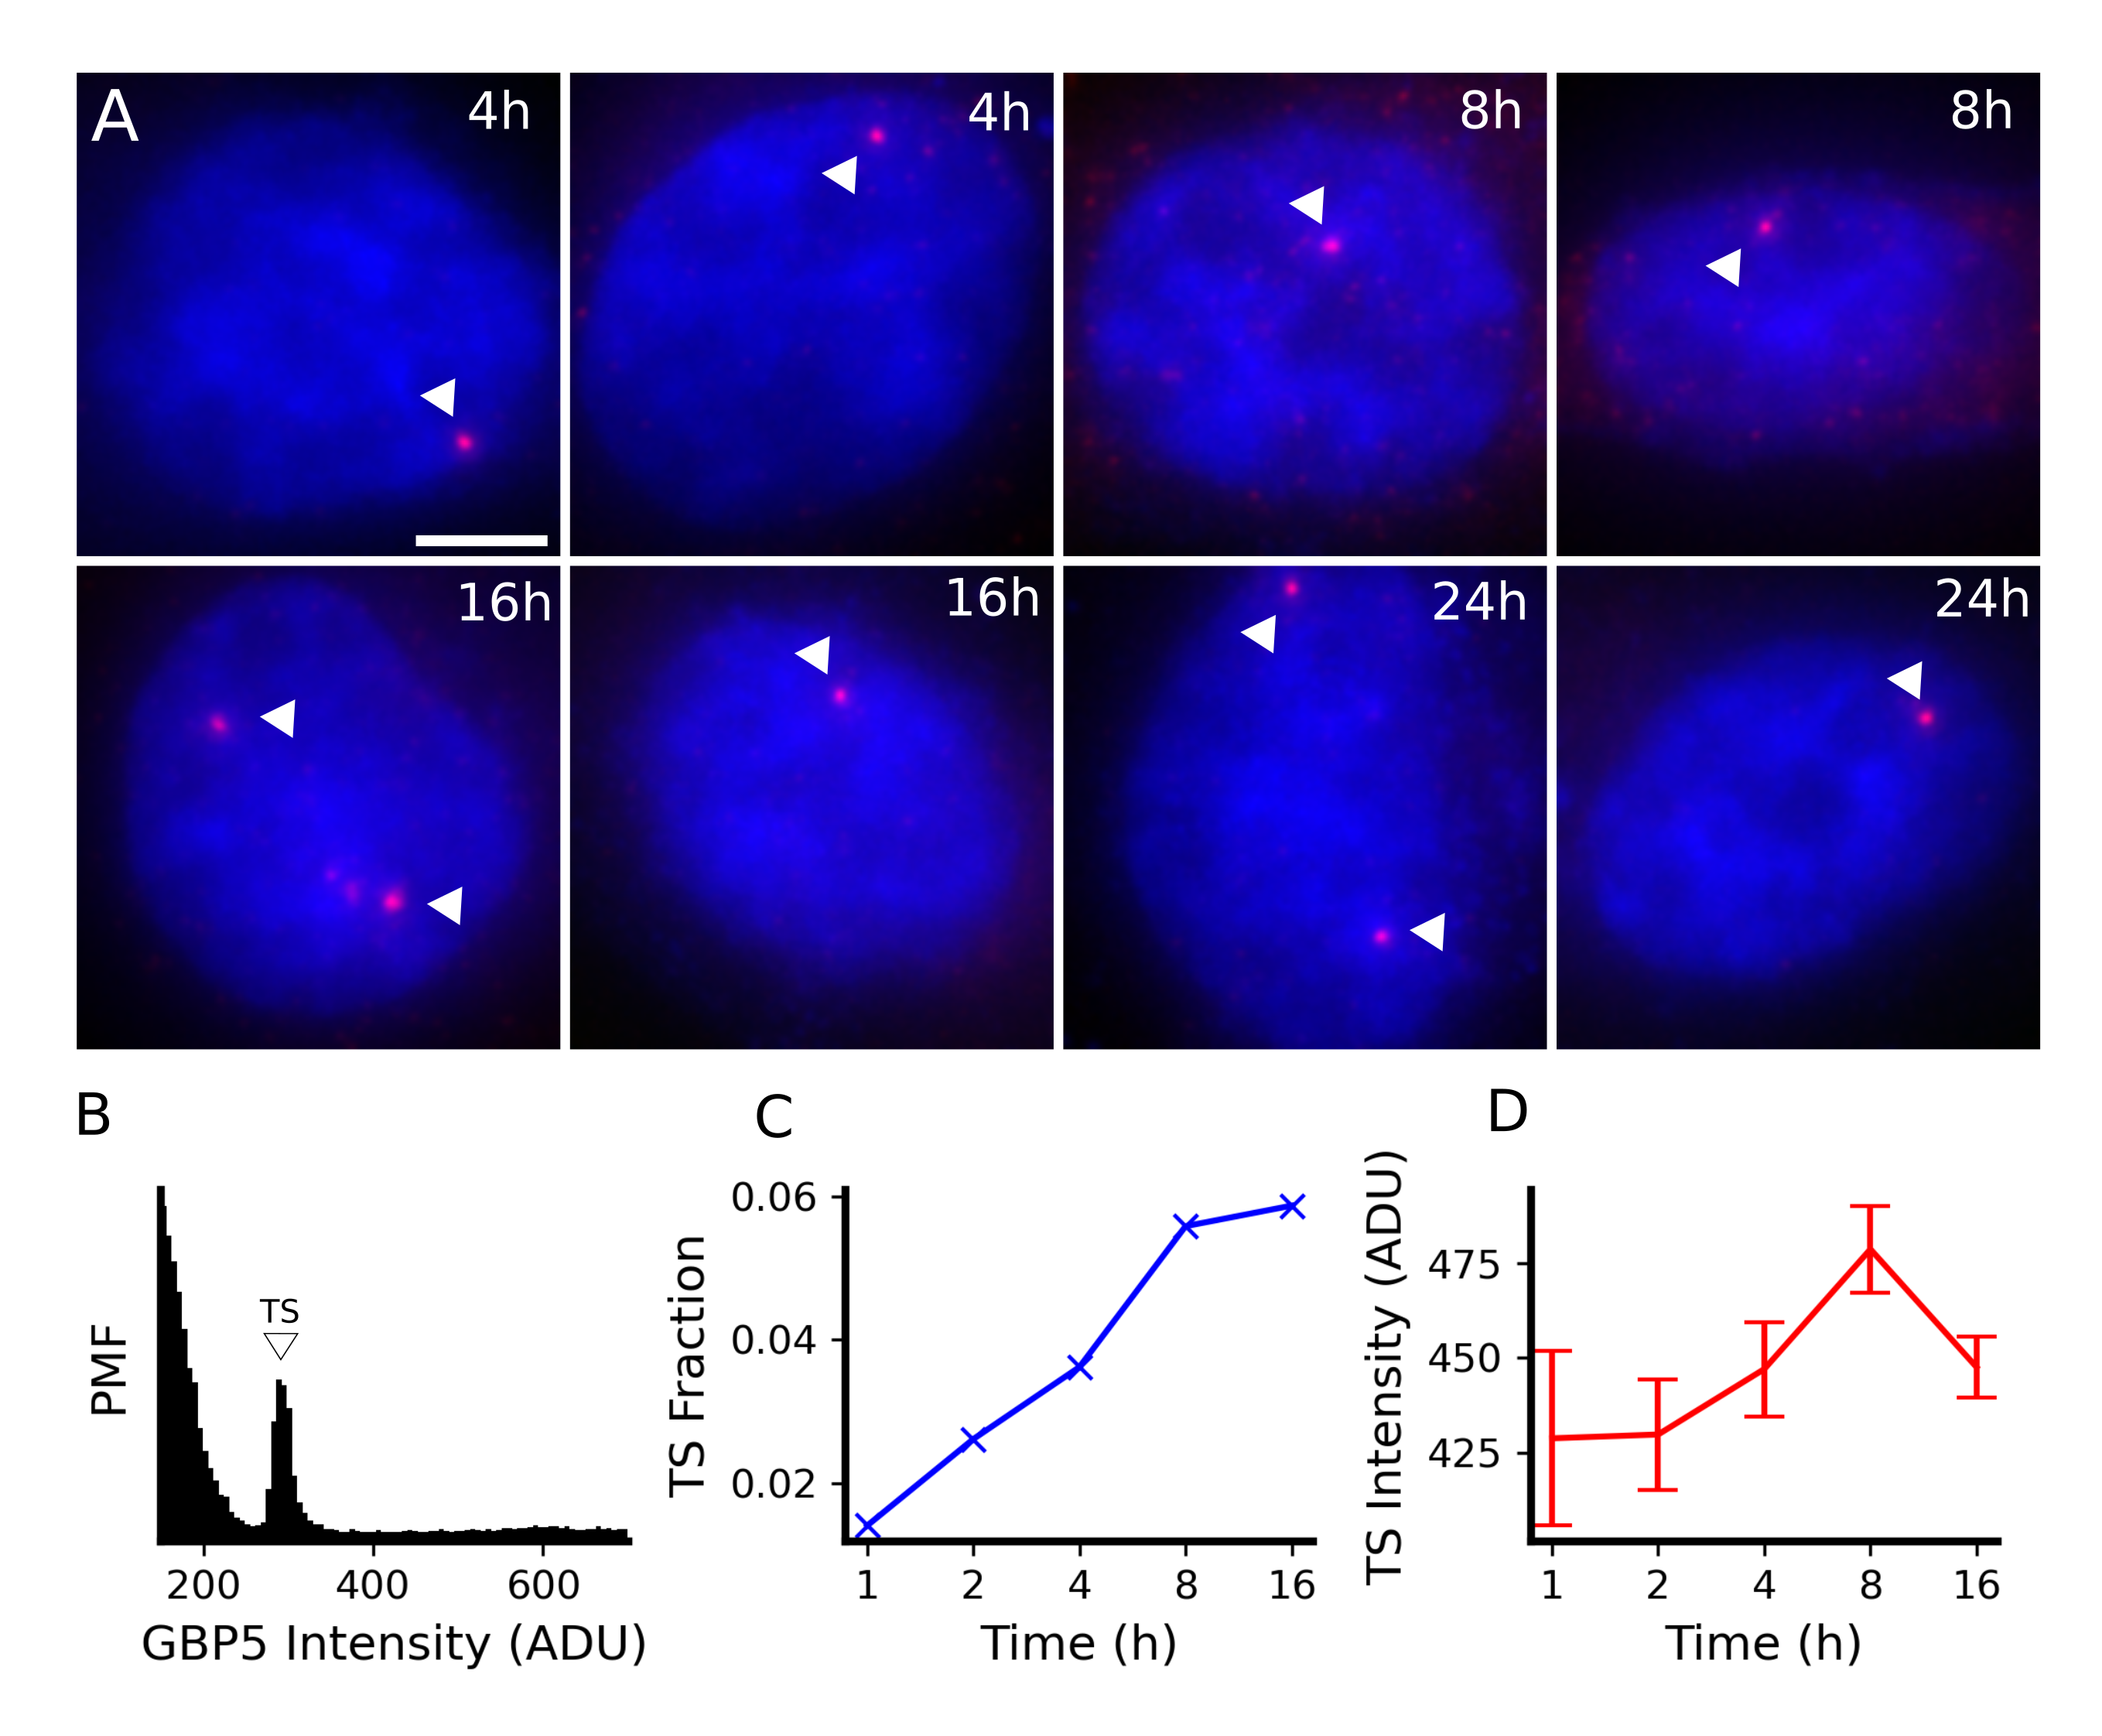
\includegraphics[width=11cm]{Figure-2.png}
\end{figure}
\end{frame}


\begin{frame}{Validaton of JQ1 efficacy for BRD4 inhibition in Hela cells}
\begin{textblock*}{6cm}(1.0cm,2.0cm)
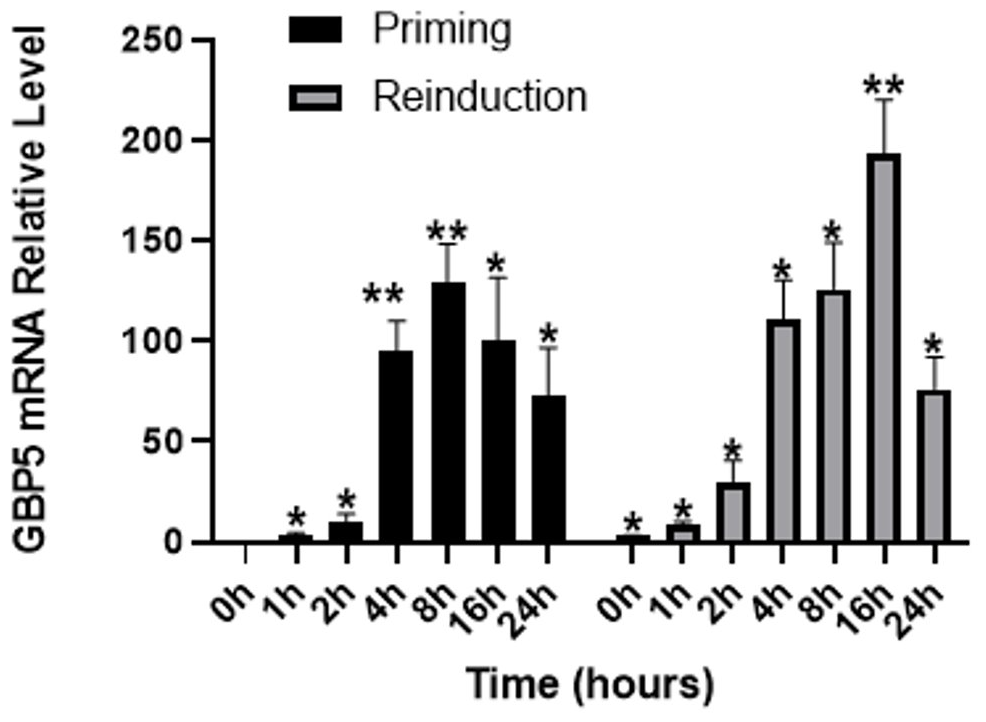
\includegraphics[width=6cm]{GBP5-RT-qPCR-crop.png}
\end{textblock*}
\begin{textblock*}{6cm}(7.0cm,2.0cm)
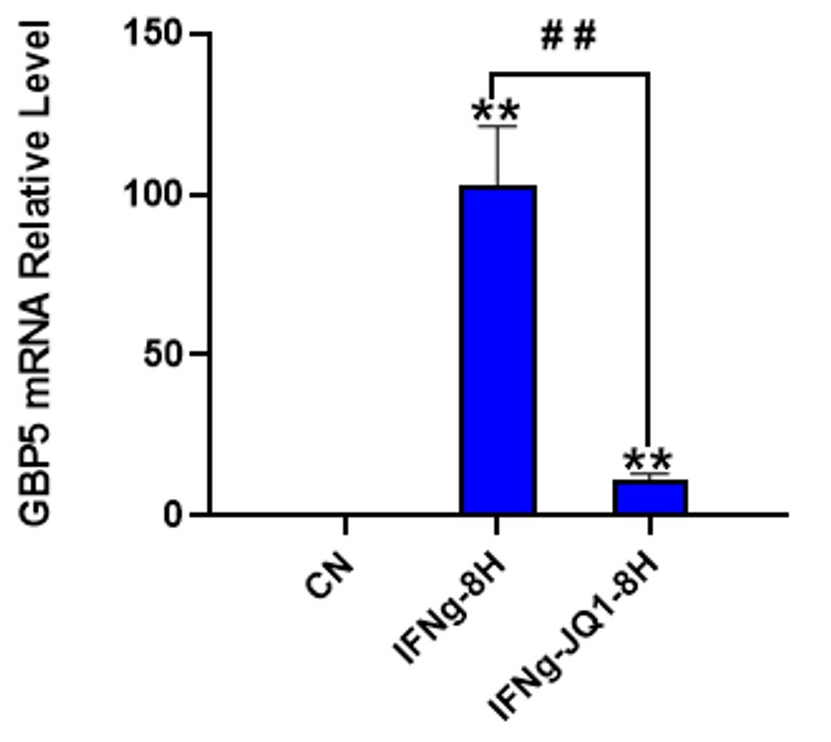
\includegraphics[width=6cm]{GBP5-JQ1-KD-crop.png}
\end{textblock*}
\end{frame}



\end{document}